\documentclass[pdflatex,compress]{beamer}

%\usetheme[dark,framenumber,totalframenumber]{ElektroITK}
\usetheme[darktitle,framenumber,totalframenumber]{ElektroITK}
\usepackage{graphicx}
\usepackage{multicol}

\title{Data Communications}
\subtitle{Data Link Control Protocols}

\author{Mifta Nur Farid}

\begin{document}

\maketitle

\begin{frame}
	\frametitle{Data Link Control Protocols}
	\begin{itemize}
		\item Requirements and objectives for effective data 		communication between two directly connected transmitting-		receiving stations:
		\begin{enumerate}
			\item Frame synchronization
			\item Flow control
			\item Error control
			\item Addressing
			\item Control and data
			\item Link management
		\end{enumerate}
	\end{itemize}
\end{frame}

\begin{frame}
	\frametitle{Flow Control}
	\begin{itemize}
		\item Technique for assuring that a transmitting entity does not over-whelm a receiving entity with data
		\begin{enumerate}
			\item The receiving entity typically allocates a data buffer of some maximum length for a transfer
			\item When data are received, the receiver must do a certain amount of processing before passing the data to the higher-level software
		\end{enumerate}
		\item In the absence of flow control, the receiver’s buffer may fill up and overflow while it is processing old data
	\end{itemize}
\end{frame}

\begin{frame}
	\begin{center}
		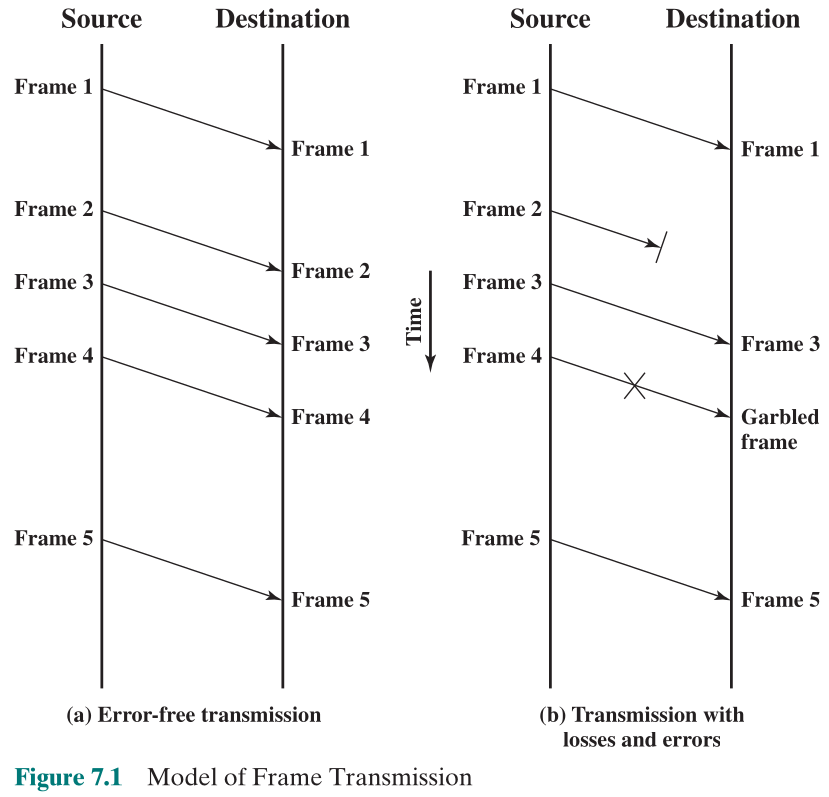
\includegraphics[width=0.6\linewidth]{img/img01}
	\end{center}
\end{frame}

\begin{frame}
	\frametitle{Stop-and-Wait Flow Control}
	\begin{itemize}
		\item Simplest form of flow control
		\begin{enumerate}
			\item Source transmits frame
			\item Destination receives frame and replies with acknowledgement (ACK)
			\item Source waits for ACK before sending next frame
			\item Destination can stop flow by not send ACK
		\end{enumerate}
	\end{itemize}
\end{frame}

\begin{frame}{Stop-and-Wait Flow Control}
	\begin{itemize}
		\item It is often the case that a source will break up a large block of data into smaller blocks and transmit the data in many frames
		\begin{itemize}
			\item The buffer size of the receiver may be limited
			\item The longer the transmission, the more likely that there will be an error, necessitating retransmission of the entire frame
			\item On a shared medium it is usually desirable not to permit one station to use the medium for an extended period, thus causing long delays at the other sending station
		\end{itemize}
	\end{itemize}
\end{frame}

\begin{frame}
	\frametitle{Tugas Mandiri}
	\begin{itemize}
		\item Stallings, W. (2014). Data and Computer Communications, 10th Edition, New Jersey: Upper Saddle River
		\begin{itemize}
			\item Chapter 6 Error Detection and Correction
		\end{itemize}
		\item Gupta, P. C. (2006). Data Communications and Computer Networks. New Delhi: Prentice Hall of India
		\begin{itemize}
			\item Chapter 5 Error Control
		\end{itemize}
		\item Tanenbaum, A. S. \& Wetherall, D. J. (2013). Computer Networks, Fifth Edition. London: Pearson.
		\begin{itemize}
			\item Section 3.2 Error Detection and Correction
		\end{itemize}
	\end{itemize}
\end{frame}

\begin{frame}
	\frametitle{Tugas Terstruktur}
	\textbf{Tampilkan Tugas 6}
\end{frame}

\end{document}
